\documentclass[a4paper,10pt]{article}

\usepackage[T1]{fontenc}
\renewcommand{\ttdefault}{pcr}

\usepackage[pdftex]{graphicx}
\usepackage{listings}

\title{Prototype A1}
\author{Alkis Gotovos}

\begin{document}
\lstset{language=Erlang, basicstyle=\small \ttfamily}

\begin{titlepage}
\maketitle
\thispagestyle{empty}
\end{titlepage}

\section{Introduction}
The aim of this document is to describe the \emph{structure} and \emph{features}
of a fully functional prototype for the Erlang concurrency testing tool that we
intend to develop. Our rationale is to use this prototype (PRA1) to gain insight
into the inner workings of our main project and detect potential pitfalls
as early as possible.

In the following sections we present the subset of functionality that we
shall implement in PRA1, as well as an overview of its architecture
(which possibly forms a structural preview for our main project).

\section{Functionality}
Being the very first prototype, PRA1 shall only implement a core subset of the
overall functionality. Specifically, we shall consider the following Erlang
"constructs" for now:
\begin{itemize}
	\item The \lstinline+spawn/1+ BIF
	\item The \lstinline+send/2+ BIF (equivalently the \lstinline+!+ operator)
	\item The simple \lstinline+receive+ expression (not containing an \lstinline+after+ clause)
\end{itemize}

The current implementation shall accept a single erlang module for analysis
and output a log, containing all possible process interleavings
with respect to the aforementioned "constructs".

\section{Instrumentation}
To be able to analyze a module we have to use wrapper functions and statements in place of
the standard Erlang ones. The easiest way to do this (without having to mess with the Erlang runtime system)
is to preprocess the module source before handing it over to the scheduler for analysis. This preprocessing
step is called \emph{instrumentation}.

Next, we present the code transformations done by the instrumenter for the three constructs mentioned above
(functions with a \lstinline+'rep_'+ prefix are custom wrapper functions).

\lstset{emph = {Function, Process, Message, Pattern1, PatternN,
                GuardSeq1, GuardSeqN, Body1, BodyN}, emphstyle = \emph}
\begin{itemize}
	\item The statement
	\begin{lstlisting}
    spawn(Function)
	\end{lstlisting}
	will become
	\begin{lstlisting}
    sched:rep_spawn(Function),
    sched:rep_yield()
	\end{lstlisting}
	
	\item The statement
	\begin{lstlisting}
    Process ! Message
	\end{lstlisting}
	will become
	\begin{lstlisting}
    sched:rep_send(Process, Message),
    sched:rep_yield()
	\end{lstlisting}
	
	\item Finally, the statement
	\begin{lstlisting}
    receive
        Pattern1 [when GuardSeq1] -> Body1;
    ...;
        PatternN [when GuardSeqN] -> BodyN
    end
	\end{lstlisting}
	will become
	\begin{lstlisting}
    sched:rep_receive(
        fun(Aux) -> receive
                        Pattern1 [when GuardSeq1] -> Body1;
                    ...;
                        PatternN [when GuardSeqN] -> BodyN
                    after 0 -> Aux()
                    end
        end),
    sched:rep_yield()
	\end{lstlisting}
\end{itemize}

\section{Structure}

\begin{figure}[htb]
	\centering
	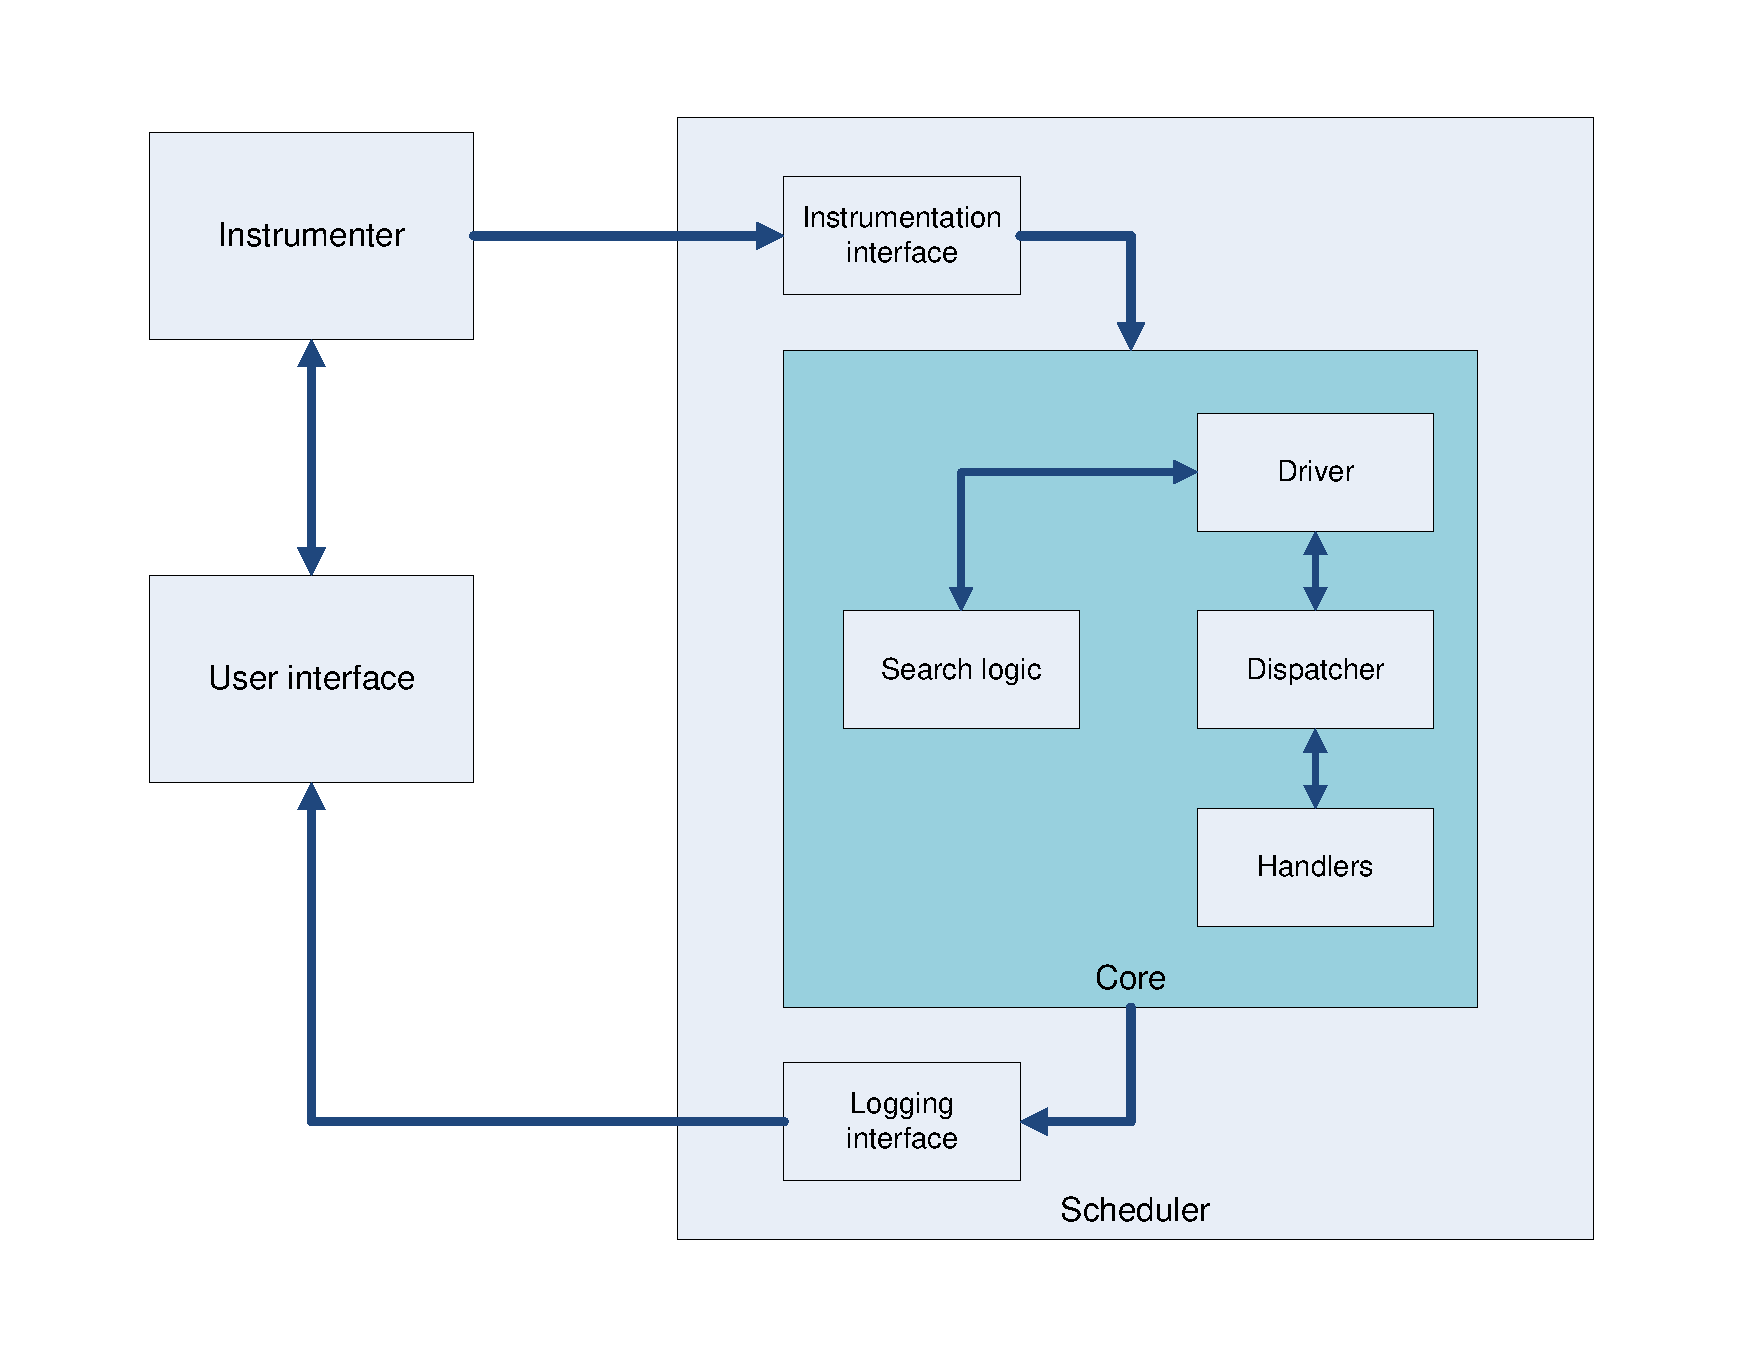
\includegraphics[width=350px]{pra1_arch}
	\caption{Architecture overview}
\end{figure}


\end{document}